\documentclass[accentcolor=tud1a, paper=a4, colorback]{tudreport}
\usepackage[utf8]{inputenc}

\usepackage{todonotes}
\usepackage[most]{tcolorbox}
\usepackage{amsmath, imakeidx, graphicx, hyperref, xcolor, float, caption}
\usepackage{chngcntr}
\counterwithout{footnote}{chapter}

%opening
\title{Flightsim Control Software Manual}
\subtitle{BP-Team 19}
\subsubtitle{Wintersemester 17/18}
\makeindex

\newcommand{\ind}[1]{#1\index{#1}}
\graphicspath{ {img/} }

\begin{document}
	\maketitle
	\tableofcontents

	\chapter*{Preamble}
	This is the manual for the flightsim control software written by the BP team 19
	of winter term 17/18. The team members are
	Frederik Bark, Heiko Carrasco, Jonas Meurer, Tim Weißmantel and Leonardo Zaninelli.
	\\
	The complete project infrastructure can be found on
	Github\footnote{\url{https://github.com/bp-flugsimulator}}.

	\chapter{Introduction}
	Using the simulator requires a lot of user inputs during start-up, due to the distributed
	nature of the infrastructure. Several programs on different computers have to be run in
	a specific order. In addition, configurations and plugins have to
	be copied to the right folders before certain programs can start. Since this is done by hand,
	usage of the simulator can be delayed depending on the simulation
	scenario and its requirements.\\
	The flightsim control software was developed to automate this cumbersome task.
	It allows running programs on
	predefined schedules and also has the ability to move files and folders prior to program
	execution.

	\section{Nomenclature}
	There are a few terms needing a more in depth definition. This section describes them in detail
	to ease the understanding of further chapters.

	\subsection{\ind{Master}}\label{master}
	Central computer, which runs the web server. Currently this is the \ind{simcontrol} computer.
	Usually the user opens the web UI on this computer, but if there is network access every other
	machine inside the institute network can be used to access the web UI. Internet access without
	a firewall should not be permitted, since there is no authentication for accessing this component.

	\subsection{\ind{Client}}
	Every computer which is part of the network, besides the master, is called a client.
	An example would be \ind{Vision}. A client can run multiple programs.

	\subsection{\ind{Program}}
	A program in this context is all software which needs to be started when the simulator is used e.g. X-Plane.
	An example for the config options of a program can be found in figure \ref{add_program}.

	\subsection{\ind{Log}}
	Some programs print their output on the command line. Since it is sometimes necessary to read
	this (e.g. for debugging purposes), every running program has a log button. Depending on the
	program (some programs do not print debugging output on the command line), the complete
	output will be shown here. The log button can be found on the program tab and can only be clicked
	when a program ran recently.

	\subsection{\ind{Files}}
	Since most simulations require a few plugins, it is possible to copy files and folders to freely
	configurable locations during a script run. An example of possible configuration options can be
	found in figure \ref{add_filesystem}.
	\\\\
	Files and folder movements are not reset automatically. For example this means that if a script copied
	a folder, the copy will stay at its new place until a manual reset is triggered by the user.

	\subsection{\ind{Script}}\label{script}
	A script is the combination of programs and file movements. It can be created by a user to model
	a scenario necessary for a simulation. The order and the needed programs and files can be configured
	freely by using the graphical editor inside the web UI.
	\\
	A script is divided into several \textit{\ind{stages}}. A stage can consist of multiple programs
	and file movements. This concept is used to make dependency management between programs easier.
	For example if  a plugin for a simulation is needed, it might be necessary to copy it before starting
	X-Plane. The plugin copy would therefore be done in stage 0 while X-Plane would be started in stage 1.
	\\\\
	Figure \ref{schedule} further illustrates this concept. This is based on the script in figure \ref{example_script}.
	After starting, the script contains one stage. All operations (starting the programs PR1 and PR2; moving files FI1 and FI2)
	are run at the same time. Afterwards, the maximum specified start time (e.g. if PR1 has a start time of 5s and FI2 has
	10s the system waits 10s) is waited. This gives a program which requires a few seconds to start sufficient time for its
	initialization.
	After the wait, the next stage is executed until there are no more stages and the script terminates.

	\begin{figure}[H]
		\centering
		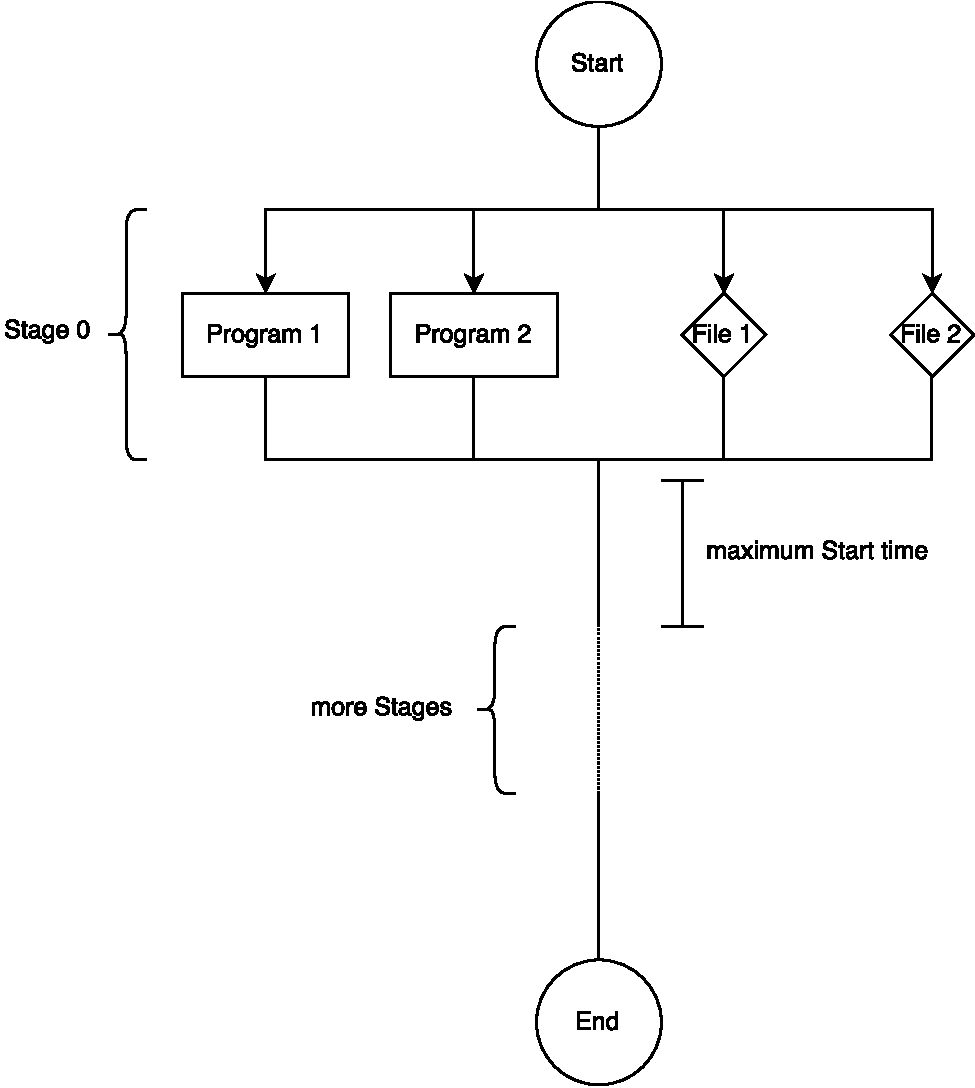
\includegraphics[width=.7\textwidth]{schedule}
		\caption{Flow Chart of a script run}
		\label{schedule}
	\end{figure}

	\subsection{Notifications}
	Some actions can trigger a notification. For example, when a client is started, a notification will be shown that
	tells the user whether the start command was send. This also happens if something goes wrong like a script crashing
	or a missing program. The color of the notification classifies it
	({\color{red}red: error}, {\color{blue}blue: info})

	\section{Project structure}
	Because of the network structure the software is build as a
	\ind{client-server system}\footnote{\url{https://en.wikipedia.org/wiki/Client-server\_model}}, which
	is outlined by figure \ref{layout_topology}.
	\begin{figure}[h]
		\centering
		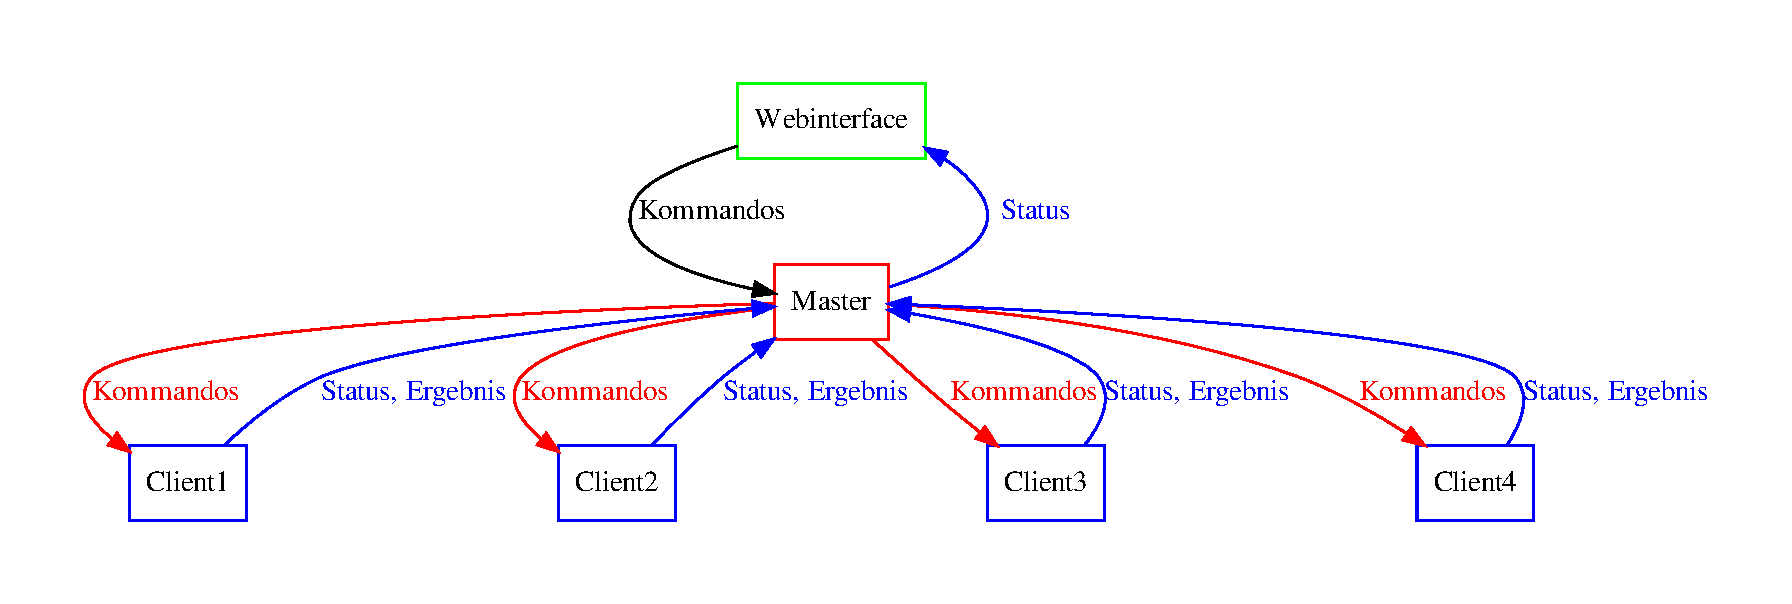
\includegraphics[width=\textwidth]{softwarelayout}
		\caption{Topology of the software layout}
		\label{layout_topology}
	\end{figure}
	\\
	The user communicates with the system using a web interface running on a computer serving as the master which
	forwards the users input to the clients.
	\\
	Both the client and the server are written in \ind{Python 3}\footnote{\url{https://www.python.org/}}.
	To shrink the necessary codebase, popular frameworks were used during development. For example,
	the website is using the \ind{Django framework}\footnote{\url{https://www.djangoproject.com/}}.
	A step by step guide for setting up the master software can be found in the project repository
	\footnote{\url{https://github.com/bp-flugsimulator/server/blob/master/README.md}}.
	\\
	The client software is also written in Python and does not need any configuration besides the address of
	the master server during startup. All further configuration is then handled by the master.


	\chapter{Installation}
	The up to date installation instructions for the server and the client can be found in the repositories.
	\section{Server}

	\begin{enumerate}
		\item Install python 3.4 or newer and git
		\item Clone the Github repository:\\ \fbox{\texttt{git clone https://github.com/bp-flugsimulator/server.git}}
		\item Run the deploy command which will setup the server and output a zip file with all relevant files:\\\fbox{\texttt{cd server \\ python manage.py deploy}}
		\item Unzip the resulting file to the desired installation directory (the cloned repository can be deleted at this point) 
		\begin{itemize}
			\item Linux:\\ \fbox{\texttt{mkdir /home/fsim-user/fsim-master \\ unzip ../server.zip /home/fsim-user/fsim-master/}}
			\item Windows: Use the Windows Explorer
		\end{itemize}
	\end{enumerate}

	\section{Client}
	\begin{enumerate}
		\item Install Python 3
		\item Open a cmd/terminal
		\item Create and navigate to the install directory \\{\color{red}(Attention! Spaces in this path can lead to unexpected behavior during runtime)}
		\begin{itemize}
			\item On Windows: \\\fbox{\texttt{md C:\textbackslash fsim-client \\ cd C:\textbackslash fsim-client\textbackslash}}
			\item On Linux/mac os: \\\fbox{\texttt{mkdir /home/fsim-user/fsim-client \\ cd /home/fsim-user/fsim-client/}}
		\end{itemize}
		\item Download the Client in one of the following ways:
		\begin{enumerate}
			\item Clone the repository from Github (Requires that git is installed):\\\fbox{\texttt{git clone https://github.com/bp-flugsimulator/client}}
			\item Download it from a running server instance from the local network:\\ To use this option the file install.py is needed from the repository. The example is given with a sever with the ip 0.0.0.0 on port 4242.\\ \fbox{\texttt{python install.py --download-client 0.0.0.0:4242}}
		\end{enumerate}
		\item Install the python dependencies with install.py (which comes with the client files):\\ \fbox{\texttt{python install.py}}
	\end{enumerate}

	\chapter{Workflows}
	\section{Adding a client}
	After starting the web server, the UI has to be opened in a browser.
	If you work on \ind{simcontrol}, just type \url{http://localhost:8000/slaves} inside
	your browser. If you are using a different computer inside the network, you
	have to replace \texttt{localhost} with the IP address of simcontrol.
	\\
	\begin{figure}[h]
		\centering
		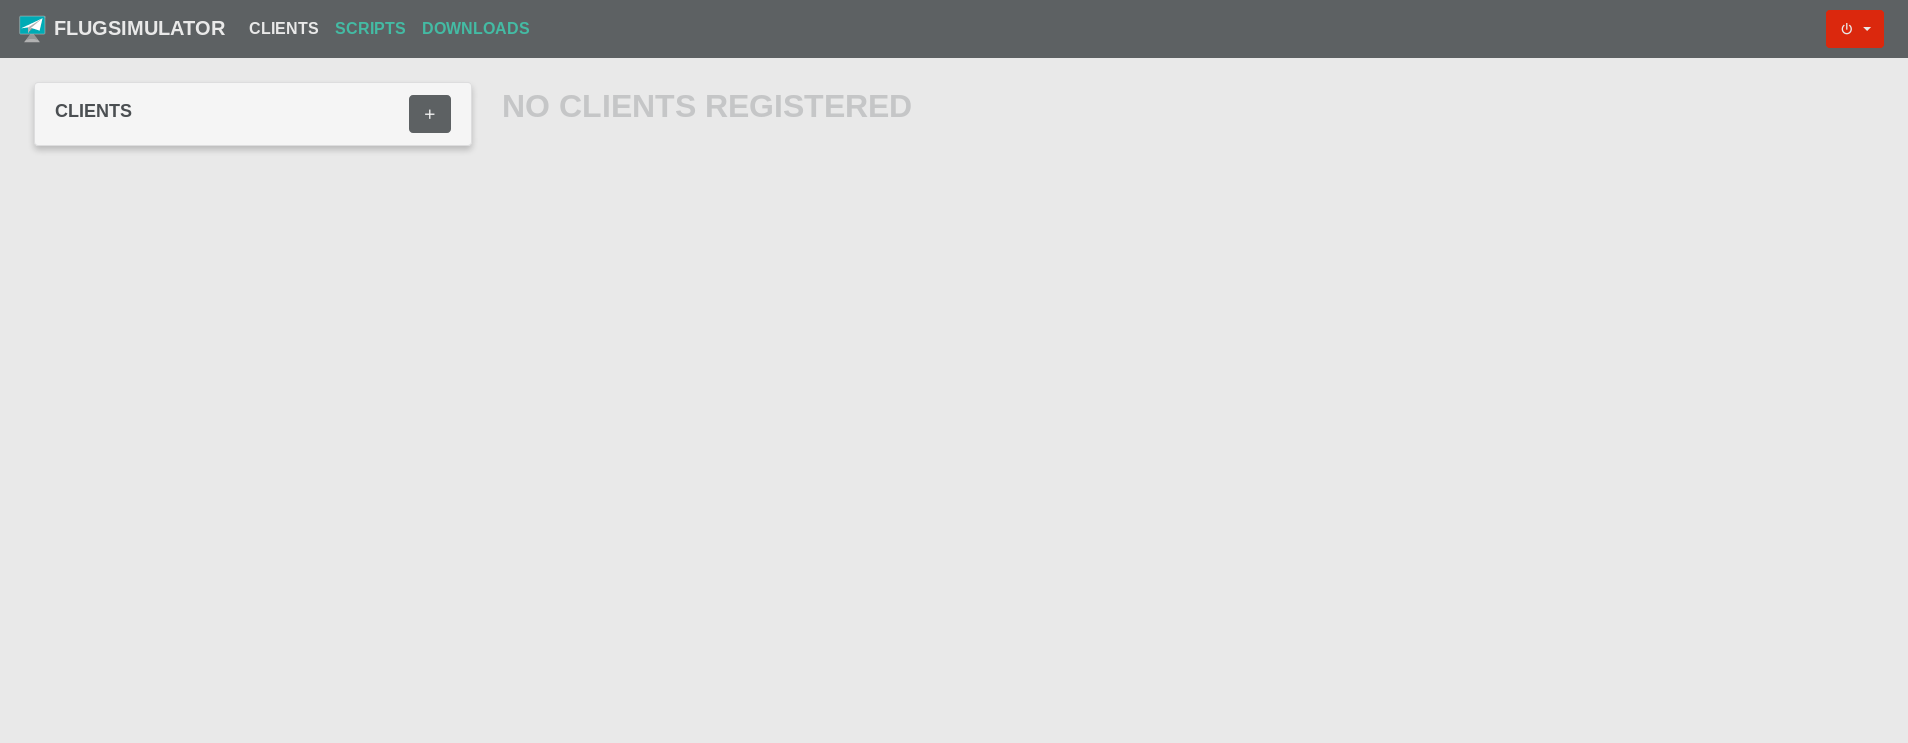
\includegraphics[width=.9\textwidth]{empty_startpage}
		\caption{The software without any configured clients}
		\label{empty_startpage}
	\end{figure}
	Adding a new client is done by clicking the \texttt{+} button in the
	client header on the left side.
	The necessary parameters are a name, an IP address,
	and a MAC address. When using a Windows client, the last two can be retrieved using
	the command \texttt{ipconfig}. Otherwise the command \texttt{ip a} can be used.
	The name is only used for the user interface
	and can be set freely.
	\\
	After creation a new client, it appears on the left sidebar. Clicking on its tab
	opens an overview with the configured programs and files for this node.
	By using the buttons \texttt{Switch On}, \texttt{Edit}, and \texttt{Delete}
	the client can be booted, deleted or its configuration can be changed.
	\section{Adding a program}
	\begin{figure}[h]
		\centering
		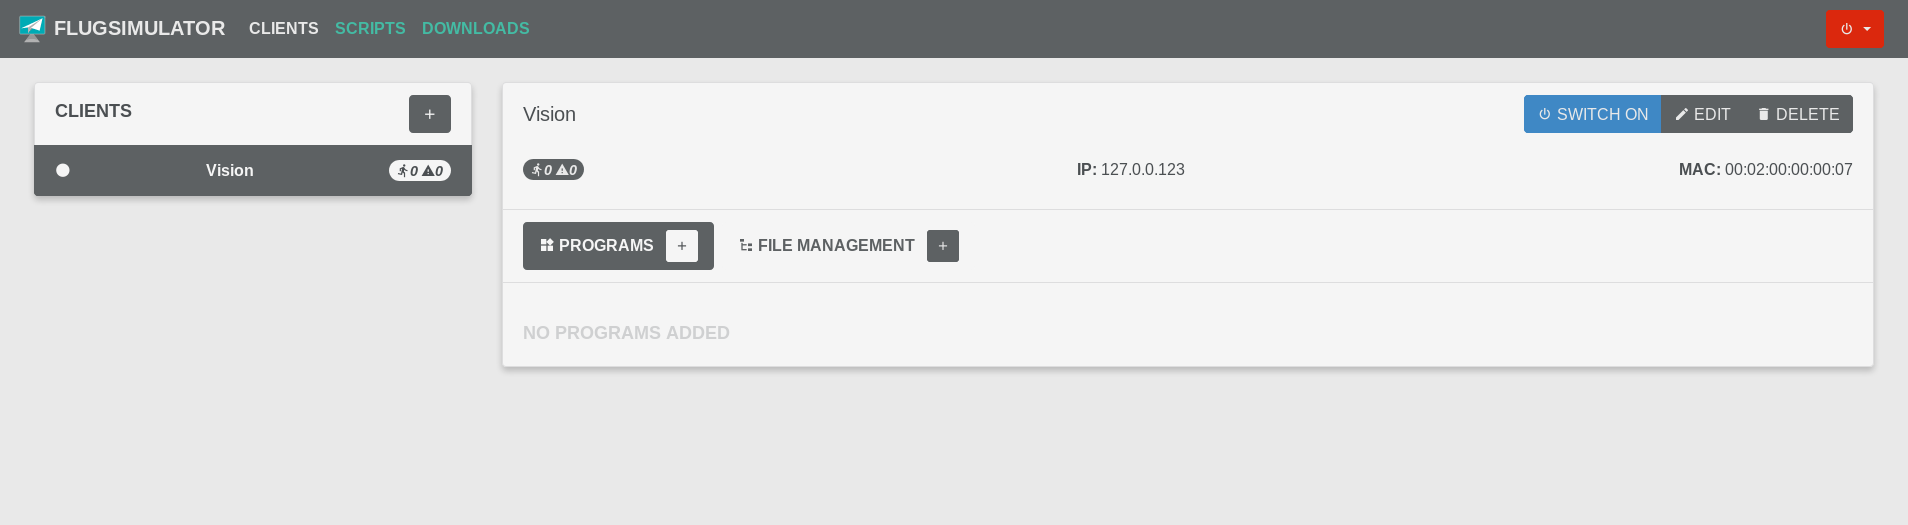
\includegraphics[width=.9\textwidth]{startpage_without_programs}
		\caption{The start page with a configured client but without any programs}
		\label{startpage_without_programs}
	\end{figure}
	To add a program, a client has to be selected first. By clicking on the \texttt{+}
	button next to the program tab, a dialog opens. The following fields can be filled
	out:
	\begin{center}
	\begin{tabular}{l|l}
		Field & Description \\\hline
		Display Name &  Display name of the program, can be chosen freely\\
		Path to Executable & Path to the executable file\\
		Arguments & Command-line arguments for the program\\
		Start time & Seconds to wait before executing the next stage during a script run\\
	\end{tabular}
	\end{center}
	"Start time" is only used during script runs.\\
	Special examples:\\
	\indent -1, the script waits for the program to terminate.\\
	\indent 0, there is no wait time after executing this program. (default)\\
	For a more complete description of stages, please look at section \ref{script}.

	\begin{figure}[h]
		\centering
		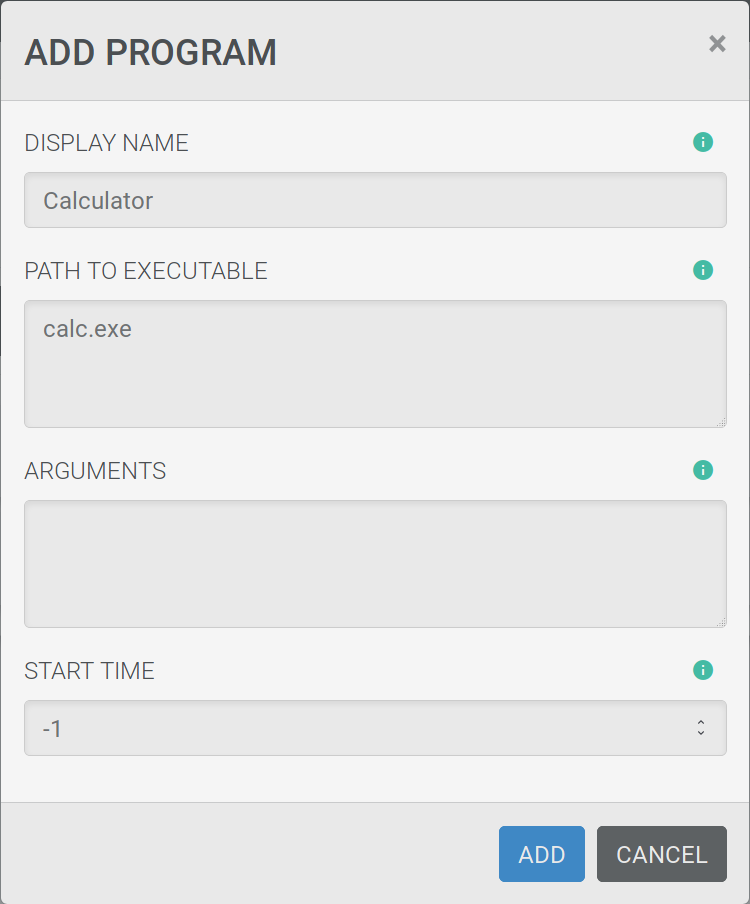
\includegraphics[width=.3\textwidth]{add_program}
		\caption{The add program dialog with example values}
		\label{add_program}
	\end{figure}

	\section{Adding a file/folder movement}

	\begin{figure}[h]
		\centering
		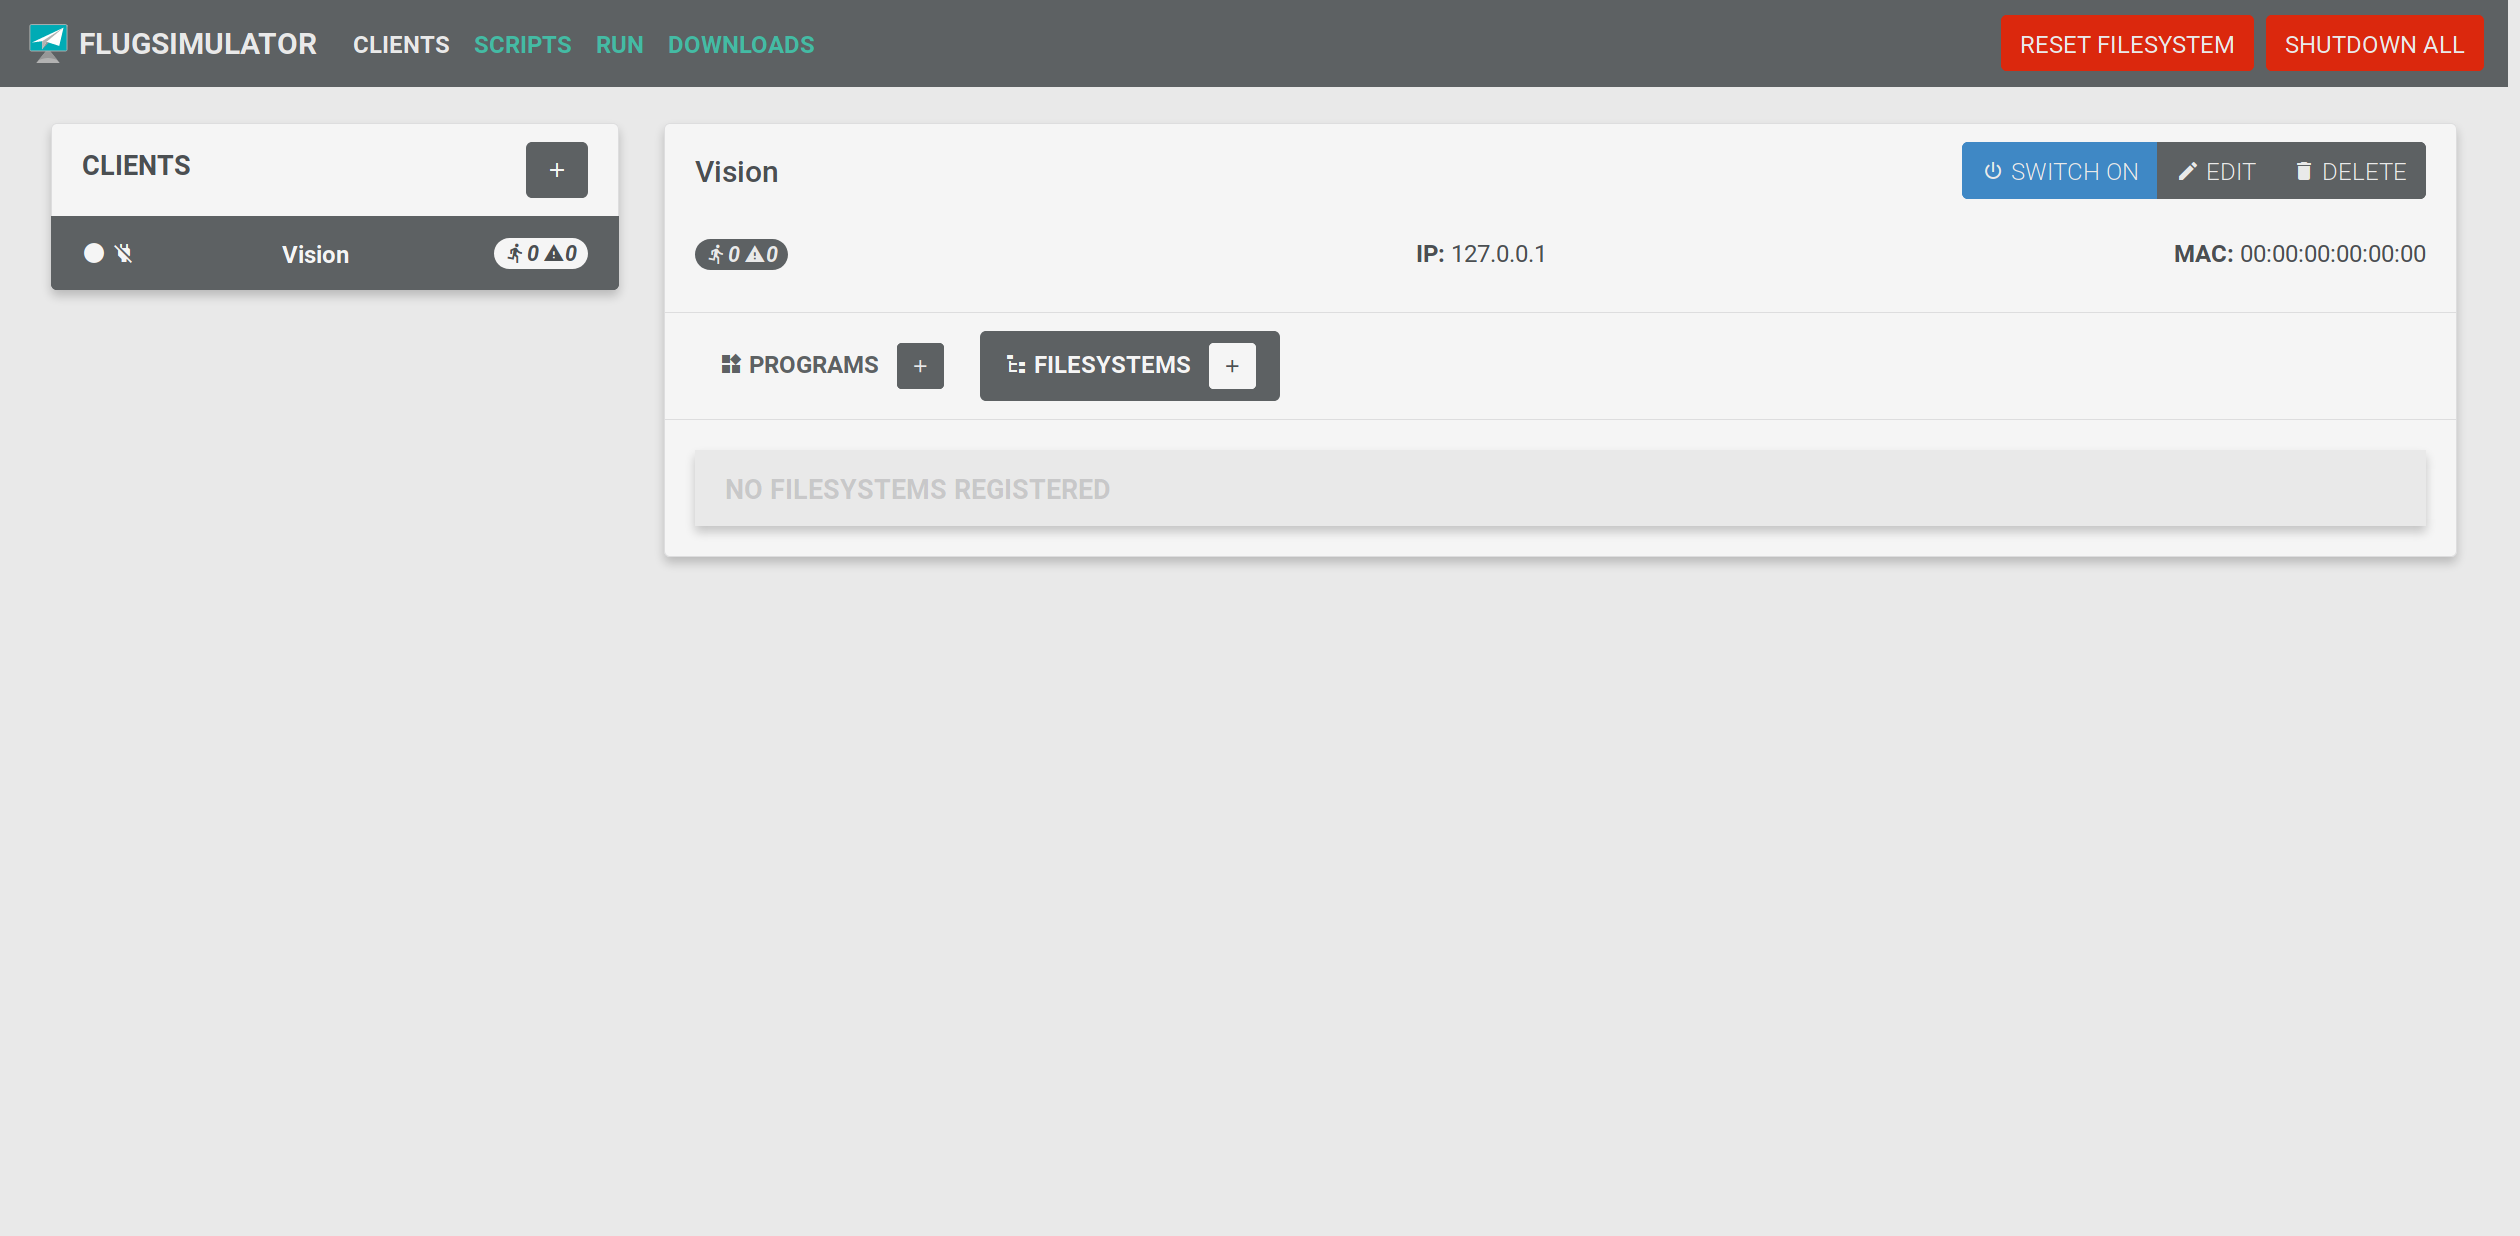
\includegraphics[width=.9\textwidth]{startpage_without_files}
		\caption{The start page with a configured client but without any files}
		\label{startpage_without_files}
	\end{figure}
	If a special plugin is necessary for a simulation scenario, it can be copied by using
	the file/folder movement function.
	\\
	In the client overview, a new file movement can be added by clicking the \texttt{+} button
	next to the file management button. The following fields have to be filled out:
	\\
	\begin{center}
	\begin{tabular}{l|l}
		Field & Description \\\hline
		Display Name &  Display name of the program, can be chosen freely\\
		Source Path & Path to the source file/folder\\
		Source Type & Type of the source, \texttt{File} or \texttt{Directory}\\
		Destination Path & Destination path (and/or new name)\\
		Destination Type & Copy mode, \texttt{Rename} or \texttt{Keep Name}\\
	\end{tabular}
	\end{center}
	The "Destination Type" can be one of two options: \texttt{Rename} or \texttt{Keep Name}.\\
	\texttt{Rename} renames the source object during copying. The last name in the destination path
	is the new name of the object. For example in figure \ref{add_filesystem} the folder
	"heli" will be copied and renamed to "helicopter".\\
	\texttt{Keep Name} copies the source into a subfolder. In the figure this would mean that
	a new folder "heli" would be created and the contents of the source will
	be copied inside it.

	\begin{figure}[h]
		\centering
		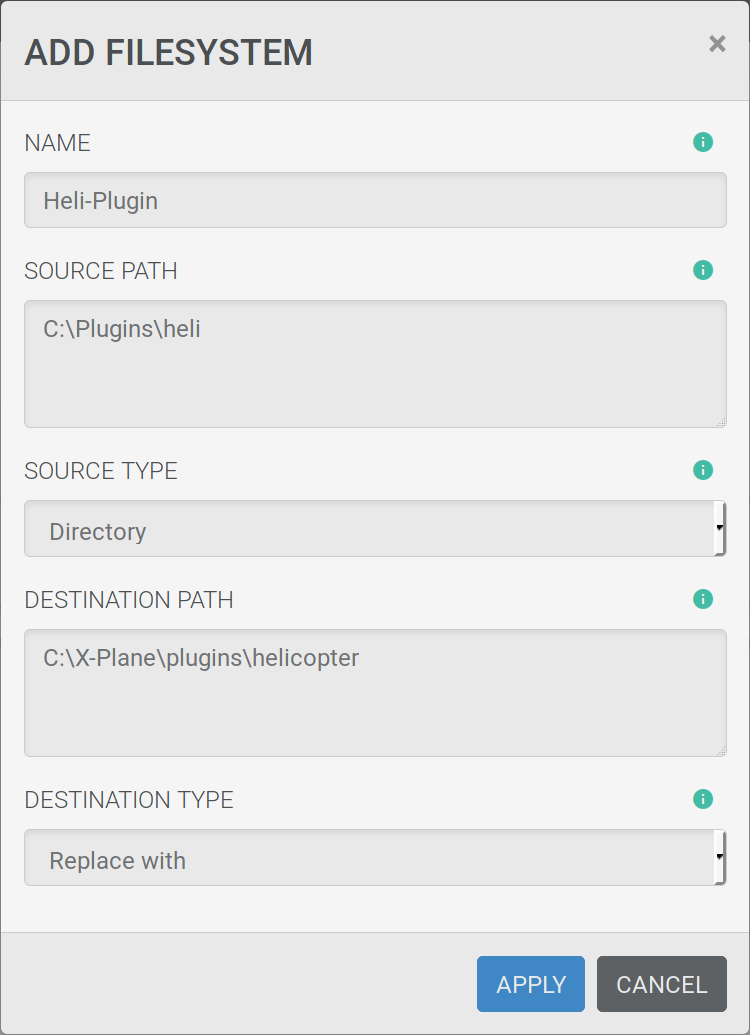
\includegraphics[width=.3\textwidth]{add_filesystem}
		\caption{The add file dialog with example values}
		\label{add_filesystem}
	\end{figure}

	\section{Adding a script}
	After adding the necessary programs and files, it is possible to create a script
	to start the simulator.
	First switch over to the Scripts tab by clicking on \texttt{Scripts}.
	All created scripts are shown in the list on the left side. An example
	without any scripts can be seen in figure \ref{scriptpage_without_scripts}.
	\begin{figure}[H]
		\centering
		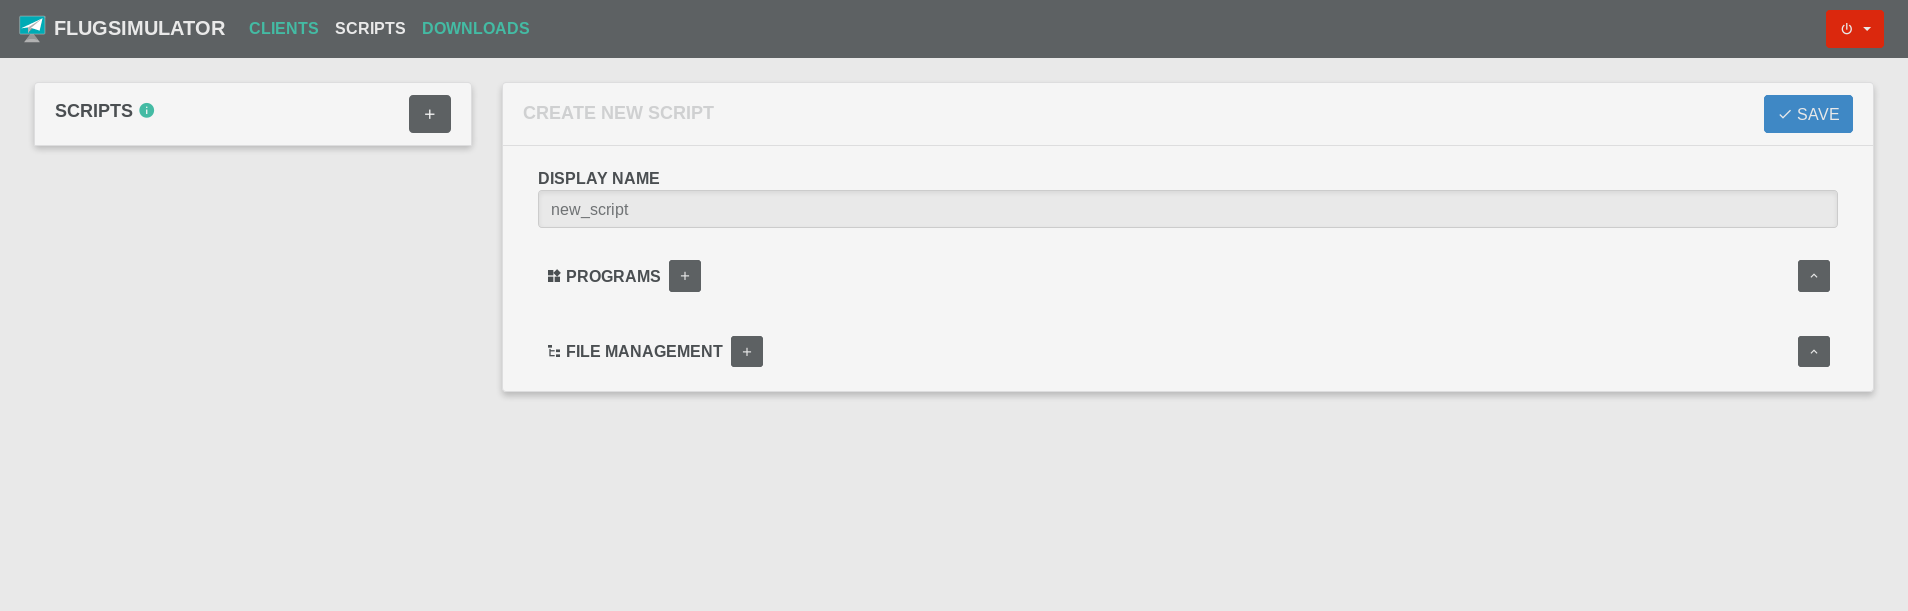
\includegraphics[width=.9\textwidth]{scriptpage_without_scripts}
		\caption{The script pages without any scripts}
		\label{scriptpage_without_scripts}
	\end{figure}
	By clicking the \texttt{+} button, a new script can be created. First, a
	display name has to be chosen. This has no other use than to help
	the user identify the script during a run.
	\\\\
	By clicking the \texttt{+} buttons next to \texttt{Programs} and \texttt{Files} it is possible
	to add new programs and files to the script. The choices "Client", "Program", and "Files" are automatically
	limited so only valid scripts can be created. The \texttt{Index} defines the stage of the
	program. It can be a natural number including zero.
	\\\\
	Wrongly entered entries can be removed by clicking the trash can. After the script is completed,
	it can be saved by clicking the \texttt{Save} button. An example for a fully functional script
	is shown in figure \ref{example_script}. A script can be copied multiple times by using
	the \texttt{Copy} button. This is particularly useful if you just want to make small modifications
	on an existing script.
	\begin{figure}[H]
		\centering
		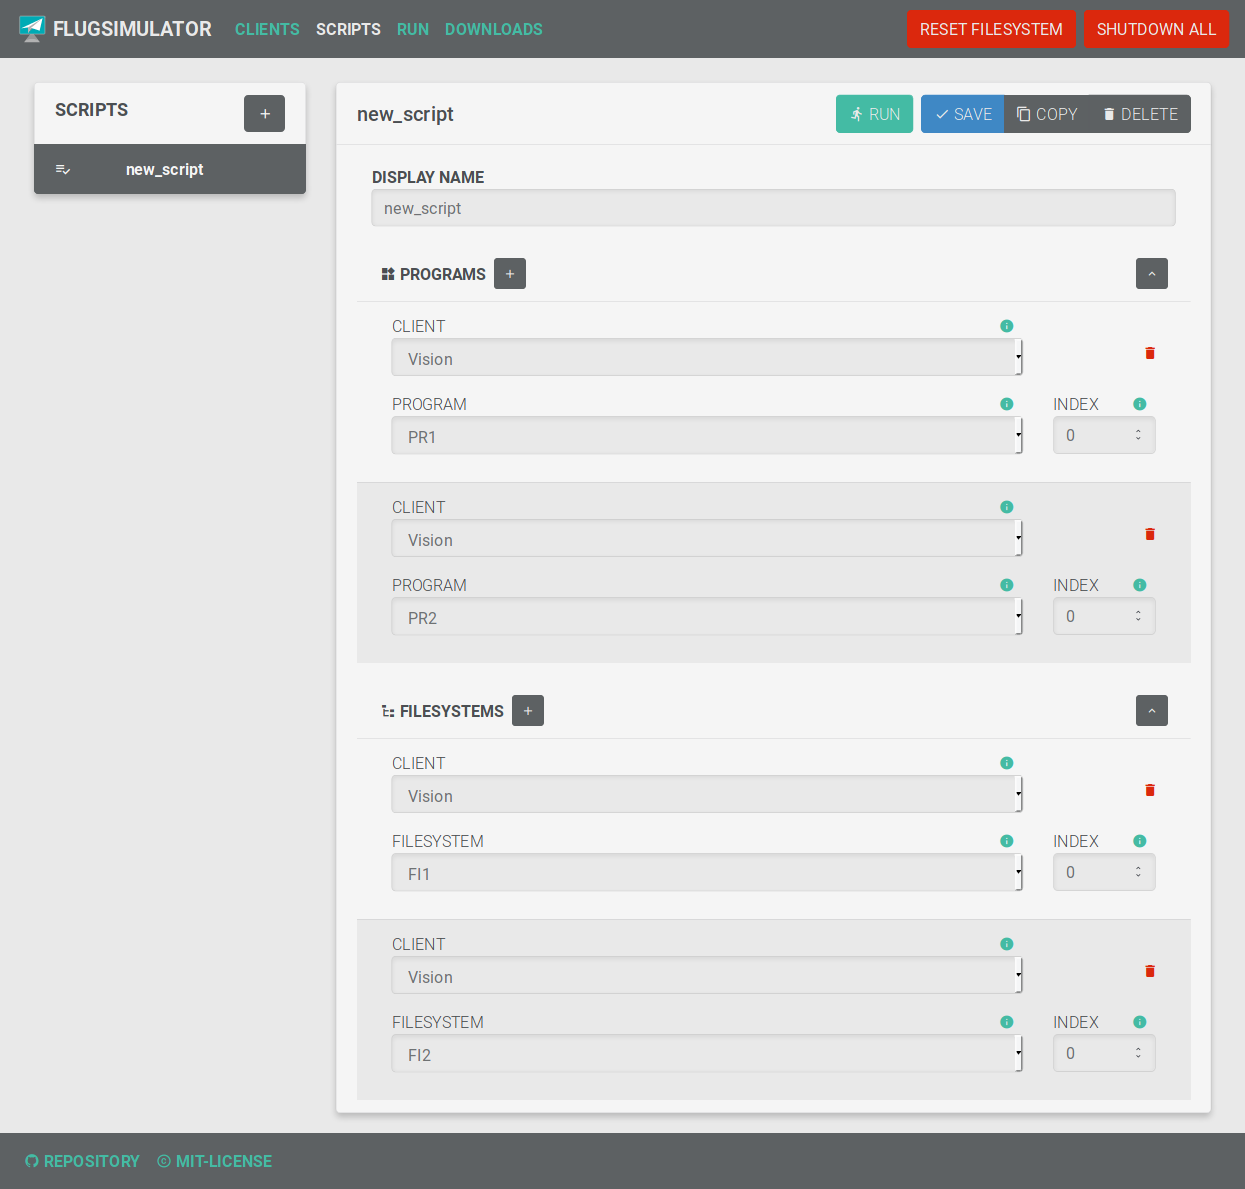
\includegraphics[width=.9\textwidth]{example_script}
		\caption{An example script}
		\label{example_script}
	\end{figure}

	\section{Running a script}
	Select a script on the script tab and click run. An overview is displayed, showing
	the script in stage form.
	\begin{figure}[H]
		\centering
		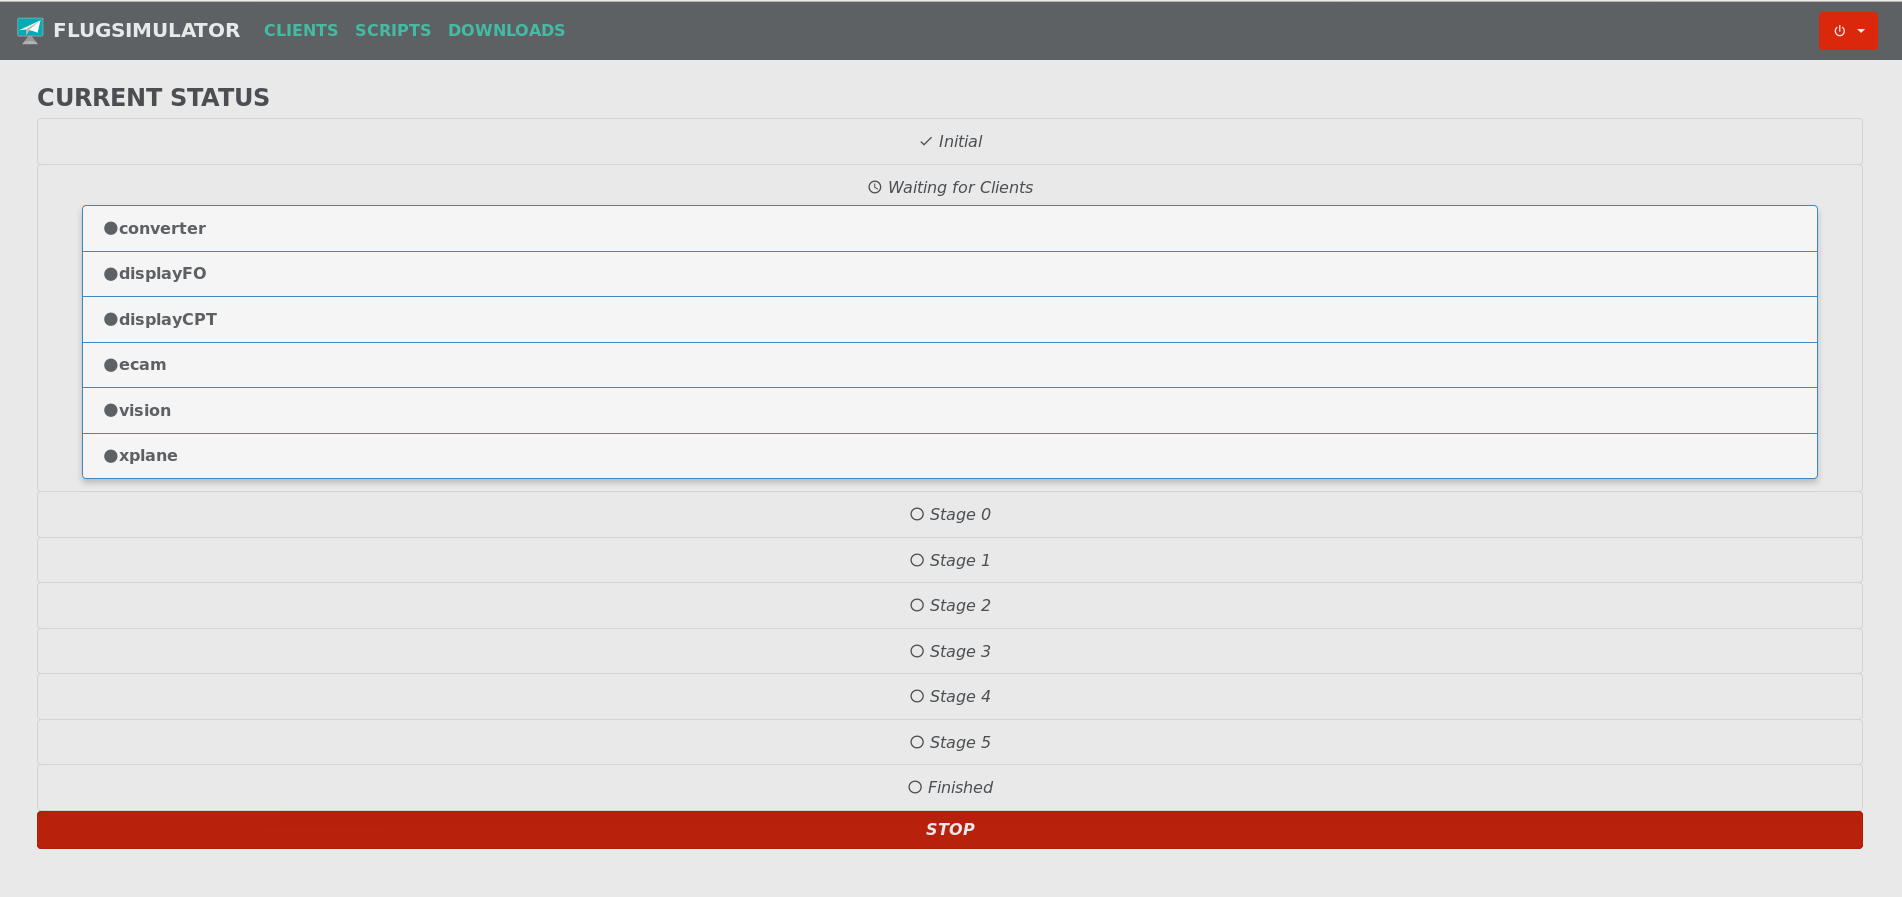
\includegraphics[width=.9\textwidth]{running_script}
		\caption{A script that is currently running}
		\label{running_script}
	\end{figure}

	\chapter{Using the simulator with scripts}
	The whole simulator can be started by switching on the master server (simcontrol).
	If there is no user interaction, the default script will be run after a short time.
	This can be prevented by using the monitor and interrupting the startup routine.
	\begin{figure}[H]
		\centering
		
\includegraphics[width=.9\textwidth]{script_run_with_timer}
		\caption{A timer showing how long it takes till the default script starts}
		\label{script_run_with_timer}
	\end{figure}
	All additional clients will be started over the network, it is not necessary to use the
	front switch on the computers.

	A user can change the default script by setting a different script to be used.
	This can be done on the edit script page.
	\begin{figure}[H]
		\centering
		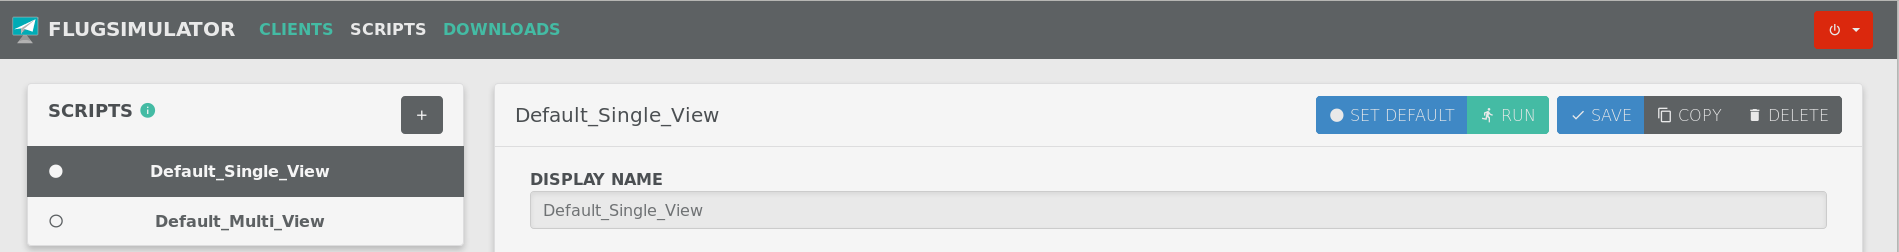
\includegraphics[width=.9\textwidth]{default_script_setting}
		\caption{The default script is set with the "set default" button}
		\label{default_script_setting}
	\end{figure}

	Usually, after working with the simulator, the whole system has to be shut down. In the top
	bar of the program there are several buttons aiding a user in stopping the system.
	\begin{figure}[H]
		\centering
		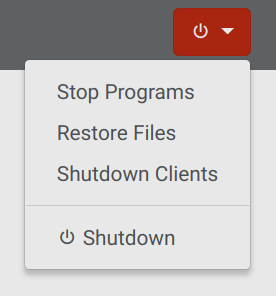
\includegraphics[width=.2\textwidth]{shutdown_dropdown_menu}
		\caption{The shutdown menu with 4 options}
		\label{shutdown_dropdown_menu}
	\end{figure}
	The options (every option will also execute the above e.g. "Restore Files" also stops all programs ["Stop Programs"]):
	\begin{itemize}
		\item "Stop Programs": All programs on every client will be terminated.
		\item "Restore Files": All moved files and directories will be restored.
		\item "Shutdown Clients": All clients will be shutdown after all programs are terminated and all files and directories are restored.
		\item "Shutdown": Additionally the master (\ref{master}) will be shutdown.
	\end{itemize}

	\section{Monitoring the system status}
	During a script run, a user can use the run script overview to monitor the status of the
	system. If more in-depth information is needed, a user can use the client overview to
	see the individual status of a client, a program, or a file/folder movement.
	Every client row contains a few buttons and status indicators, shown in figure \ref{client_status}.
	The dot on the left indicates the current client status. If the dot is
	green the client is running. The two symbols on the right of a client 
	show the number of running scripts and the amount of errors which occurred on this client.
	\begin{figure}[h]
		\centering
		
\includegraphics[width=.3\textwidth]{client_status}
		\caption{Status of the xplane client}
		\label{client_status}
	\end{figure}
	For programs and files the status bar shows a green indicator on the left during a program run as seen in figure (figure \ref{running_program}).
	\begin{figure}[h]
		\centering
		
\includegraphics[width=.6\textwidth]{running_program}
		\caption{A currently running program}
		\label{running_program}
	\end{figure}\\
	By clicking the \texttt{Log} button the current program output can be inspected.
	If the program did not shut down correctly, a red indicator is shown (figure \ref{failed_program}).
	\begin{figure}[h]
		\centering
		
\includegraphics[width=.6\textwidth]{failed_program}
		\caption{A program with a errors during shutdown or execution}
		\label{failed_program}
	\end{figure}\\

	\clearpage
	\addcontentsline{toc}{chapter}{Index}
	\printindex


\end{document}
